\documentclass[11pt]{amsart}
\usepackage{geometry}                % See geometry.pdf to learn the layout options. There are lots.
\geometry{letterpaper}                   % ... or a4paper or a5paper or ... 
%\geometry{landscape}                % Activate for for rotated page geometry
%\usepackage[parfill]{parskip}    % Activate to begin paragraphs with an empty line rather than an indent
\usepackage{graphicx}
\usepackage{amssymb}
\usepackage{epstopdf}
\usepackage{subcaption}
\usepackage{placeins}
\DeclareGraphicsRule{.tif}{png}{.png}{`convert #1 `dirname #1`/`basename #1 .tif`.png}
\graphicspath{{./notebooks/figs/}}

\title{STAT 215A, Final Project: Classifying ciTBI in Youth}
\author{Mark Oussoren, Sahil Saxena, Hyunsuk Kim, Florica Constantine}
\date{12/10/2021}                                           % Activate to display a given date or no date

\begin{document}
\maketitle


\section{Introduction}

% How can we best vet and/or improve the clinical decision rule for your given problem? Most importantly, the clinical decision rule should be highly predictive and minimize the amount of missed diagnoses (i.e. have a very high sensitivity). It should also be easy-to-use, using variables that clinicians can readily have access to when making their decisions. Finally, the interpretability of the rule helps to check whether its predictions will make sense for new patients and makes it easier to apply in new settings.

Traumatic brain injuries, hereafter referred to as TBIs, are both commonplace and require immediate medical attention. However, diagnoses often require a CT scan to confirm the presence of a TBI [CITE 14-16 from paper]. In children, this need is problematic, as the radiation from a CT scan can lead to long-term adverse affects; hence, given a child presenting with a potential TBI, it is desirable to find a way to decide whether they actually need a CT scan. Note that forgoing a CT scan in the presence of an actual TBI is also undesirable. In this report, we revisit the data from [CITE] and derive an updated decision rule for identifying which child patients need a CT scan. 

TODO: OUTLINE OF SECTIONS

\section{Data}

\subsection{Data collection}

% What are the most relevant data to collect to answer the question in (1)? Ideas from experimental design (a subfield of statistics) and active learning (a subfield of machine learning) are useful here. The above question is good to ask even if the data has already been collected because understanding the ideal data collection process might reveal shortcomings of the actual data collection process and shed light on analysis steps to follow. The questions below are useful to ask: How were the data collected? At what locations? Over what time period? Who collected them? What instruments were used? Have the operators and instruments changed over the period? Try to imagine yourself at the data collection site physically.

The authors in [CITE] collected data in a prospective cohort study from 43,499 patients younger than 18 years of age that visited a hospital within 24 hours of experiencing head trauma. The study was run across 25 pediatric emergency departments over a span of approximately 2 years, where the last few months were used to collect samples for validating the decision rules derived in the original study. Only patients with GCS (Glasgow Coma Scale) scores of 14 or 15 were considered; those with scores 13 or less were enrolled but were not grouped with the others. For each patient, a trained investigator or other medical personnel recorded various prespecified details, e.g., mechanism of injury, medical history, and responses to standardized questions about the presence of several symptoms or signs of head trauma on a standardized data form. For a small subset of patients (approximately 4\%), a second assessment was performed for quality control purposes--note that we do not use this information, but that its presence is reassuring. 

\subsection{Meaning}

% What does each variable mean in the data? What does it measure? Does it measure what it is supposed to measure? How could things go wrong? What statistical assumptions is one making by assuming things didn’t go wrong? (Knowing the data collection process helps here.) Meaning of each variable -- ask students to imagine being there at the ER and giving a Glasgow coma score, for example, and also a couple of variables -- ask students what could cause different values written down. How were the data cleaned? By whom?

The study defined death, prolonged hospital admission or intubation, or the need for surgery following a CT scan as a positive, ciTBI outcome. Other patients were assigned to the negative outcome; to find missed positives, the study coordinators performed telephone surveys to follow up with parents and tracked followup visits. If a positive outcome was missed, the patient's label was updated to positive. 

An important variable in this data set is the GCS score. The Glasgow Coma Scale is a common scoring system used in emergency departments to determine a patient's level of consciousness by rating their ability to pass certain tests for eye and motor movement along with verbal ability. The scores from each of these three categories are summed to form a total GCS score. The lower the score a patient has in each category leads to a lower GCS total score (meaning the worse a state a patient is in). A GCS score ranges from 3-15.

Note that several variables or descriptors in the study require the ability to converse with the child for assignment, e.g., the presence of a headache or whether or not the child is suffering from amnesia. Similarly, a GCS score for a pre-verbal child is also calculated by slightly different metrics than those for an adult. Judging verbal ability, especially, is different with a condition like "inappropriate words" being instead assessed as "cries to pain" for those children who are pre-verbal. Even motor ability has some conditions assessed differently such as looking for "spontaneous
movement" rather than "follow commands" in preverbal children. Hence, both the authors of [CITE] and us chose to separate patients under the age of two (pre-verbal) from those aged two or older (verbal) in their analysis. Moreover, as children under the age of two are more sensitive to radiation, it is reasonable to consider this group separately [CITE SOMETHING]. Note that this is not a perfect grouping as some children will be verbal by age two and some children are not verbal after age 2 but, nonetheless, it is good developmental benchmark [CITE SOMETHING].

The variables in our data are all categorical or ordinal, except for age (however the categorial version of the age variable where it was discretized by $< 2$ years old and $\geq 2$ years old was used in all our analyses for the reasons stated above). It would be ideal if instead the continuous version of the variables were reported and they were not pre-sorted into sometimes arbitrarily chosen categories (i.e. the length of a seizure is binned as  $< 1$ min, $1 - 5$ min, $5 ‐ 15$ min, and $> 15$ min).

Other important variables included in our data set are the injury mechanism, injury severity, and whether the child is acting normally, is intubated, is paralyzed, and/or is sedated.

Several binary indicator variables exist looking at, respectively, whether a child suffered a loss of consciousness, seizure, headache, vomiting, altered mental state, palpable skull fracture, basilar skull fracture, hematoma, trauma above the clavicles, neurological deficits, or other (non-head) substantial injuries. Each of these variables also has more specific follow up questions, e.g. the type of basilar skull fracture if it is indicated a patient has one.

Lastly, we also have several meta variables such as patient number, race, ethnicity, gender, position of medical professional, and certification of medical professional. These variables do not affect whether a patient will be positive for ciTBI. However, they may be useful to look at after our analyses are complete in cases they are acting as a proxy for something deeper that is taking place but should not be used as feature inputs to our models.

\subsection{Exploratory Data Analysis}

\subsubsection{Outcome}

First, we looked at our outcome variable and noted that there were 20 patients that had a missing value. Note, there is a discrepancy where with [CITE], where they mention 18 not 20 patients have a missing value. However, the reasoning for this difference could not be resolved. Of these 20 patients, 17 of them are negative for all four of the variables making up our outcome (death, hospital admission of longer than 2 days post CT, intubation for more than 24 hours, or neurological surgery). We thus assign these patients as being negative for a ciTBI. For two of the three remaining patients they are negative for three of the variables and only have death because of TBI missing. The last remaining patient has missing values for intubation and death by TBI. We impute all three of these patients to also be negative for ciTBI after talking to our clinician collaborators who suggest it is unlikely death by TBI or intubation would not be marked on a medical form if they did in fact take place. The proportion of each of the four outcomes is shown below in Figure \ref{fig:outcome_type}. We can see that the vast majority of people were positive for a prolonged hospital stay.
\FloatBarrier
\begin{figure}
	\centering
	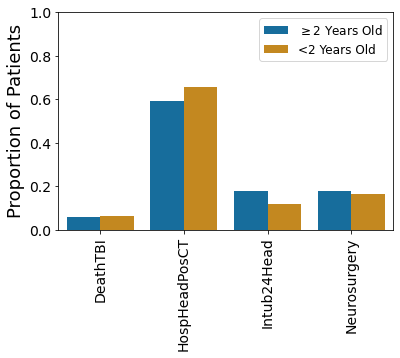
\includegraphics[width=0.5\textwidth]{outcome_type.png}
	\caption{Outcome Type}\label{fig:outcome_type}
\end{figure}
\FloatBarrier

\subsubsection{GCS Scores}

From [CITE], we learned that it is not controversial to perform a CT scan for patients with a GCS score ranging from 3 to 13 as in this group the risk of finding a TBI on a CT is more than 20\%. For our data set, we looked at the proportion of patients positive for ciTBI with a GCS scores in the range of 3-13 and also for those in the range for 14-15 in Figure \ref{fig:GCSClass}. Looking at this we can see that 40\% of patients with a GCS score in the range of 3 to 13 were positive for ciTBI versus only 0.8\% of those with a GCS score of 14 or 15. This is quite a dramatic difference. However, we wanted to know if separating the GCS score into classes with a cutoff GCS score of 14, in particular, was the best possible split. We broke up the previous plot further into individual GCS scores (Figure \ref{fig:GCSTotal}). We can see that, in general, the lower the GCS score the higher the proportion is for a patient to be positive for ciTBI, as expected. Even at a GCS of 13, 20\% of patients were positive for ciTBI. Thus, keeping the current cutoff of 3-13 and 14-15 as the two separate GCS classes seems reasonable. We remove any patients from here on out that have a GCS in the range of 3-13 (969 total patients) as the risk of having a positive ciTBI is too high and any decision rule would suggest always performing a CT scan for this group.
\FloatBarrier
\begin{figure}
	\begin{minipage}[b]{0.5\linewidth}
		\centering
		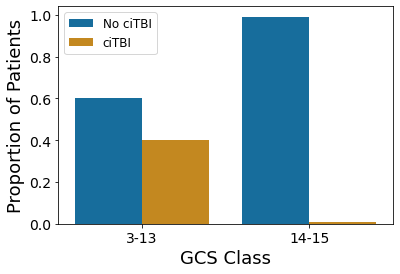
\includegraphics[width=\textwidth]{GCSClass_prop.png}
		\subcaption{GCS Class}\label{fig:GCSClass}
	\end{minipage}%
	\begin{minipage}[b]{0.5\linewidth}
		\centering
		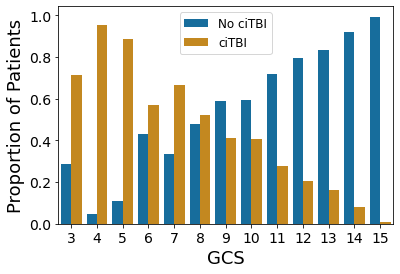
\includegraphics[width=\textwidth]{GCSTotal_prop.png}
		\subcaption{GCSTotal Score}\label{fig:GCSTotal}
	\end{minipage}
	\caption{GCS Figure}\label{fig:GCS}
\end{figure}
\FloatBarrier

\subsubsection{Data Missingness}

Next we look at the rate of missingness for each feature in Figure \ref{fig:cov_missing}. We note that the features "Dizzy" and "Ethnicity" are missing in more than 35\% of patients. On the data form, ethnicity asks whether the patient is hispanic or not and may potentially be skipped over by a patient if they fill in the race field instead (or if they are too young to fill out a form and the medicial personnel does not want to guess). However, we are already considering ethnicity to be a meta variable and did not use it in our analyses anyway. After speaking with the clinicians, we learned that notating whether a patient is dizzy or not is not very relevant in diagnosing TBI and it is also a very subjective variable as it is highly susceptible to change from patient to patient based on their own personal definition of feeling dizzy. 

For the other variables with missingness, they were either imputed with what a `healthy' response would be, e.g. a `No' value would be imputed for missing paralyzed or sedated values. Otherwise, the response that was the mode was used for variables where there is no clear `healthy' response. e.g. hematoma size, number of times a patient vomited.

Many variables have a parent question such as `Seiz' for seizure that have follow up question such as the length of the seizure. If a patient has a response of `No' for seizure then in the form `Not applicable' is often marked for each follow up question. We convert these `Not applicable' answers to be `No' to make analyses easier to perform.

We further note that the majority of patients have only around 1\% of data features missing, and at most still under 20\% (Figure \ref{fig:sample_missingness}) and thus we do not drop any patients from our analyses.
\FloatBarrier
\begin{figure}
	\centering
	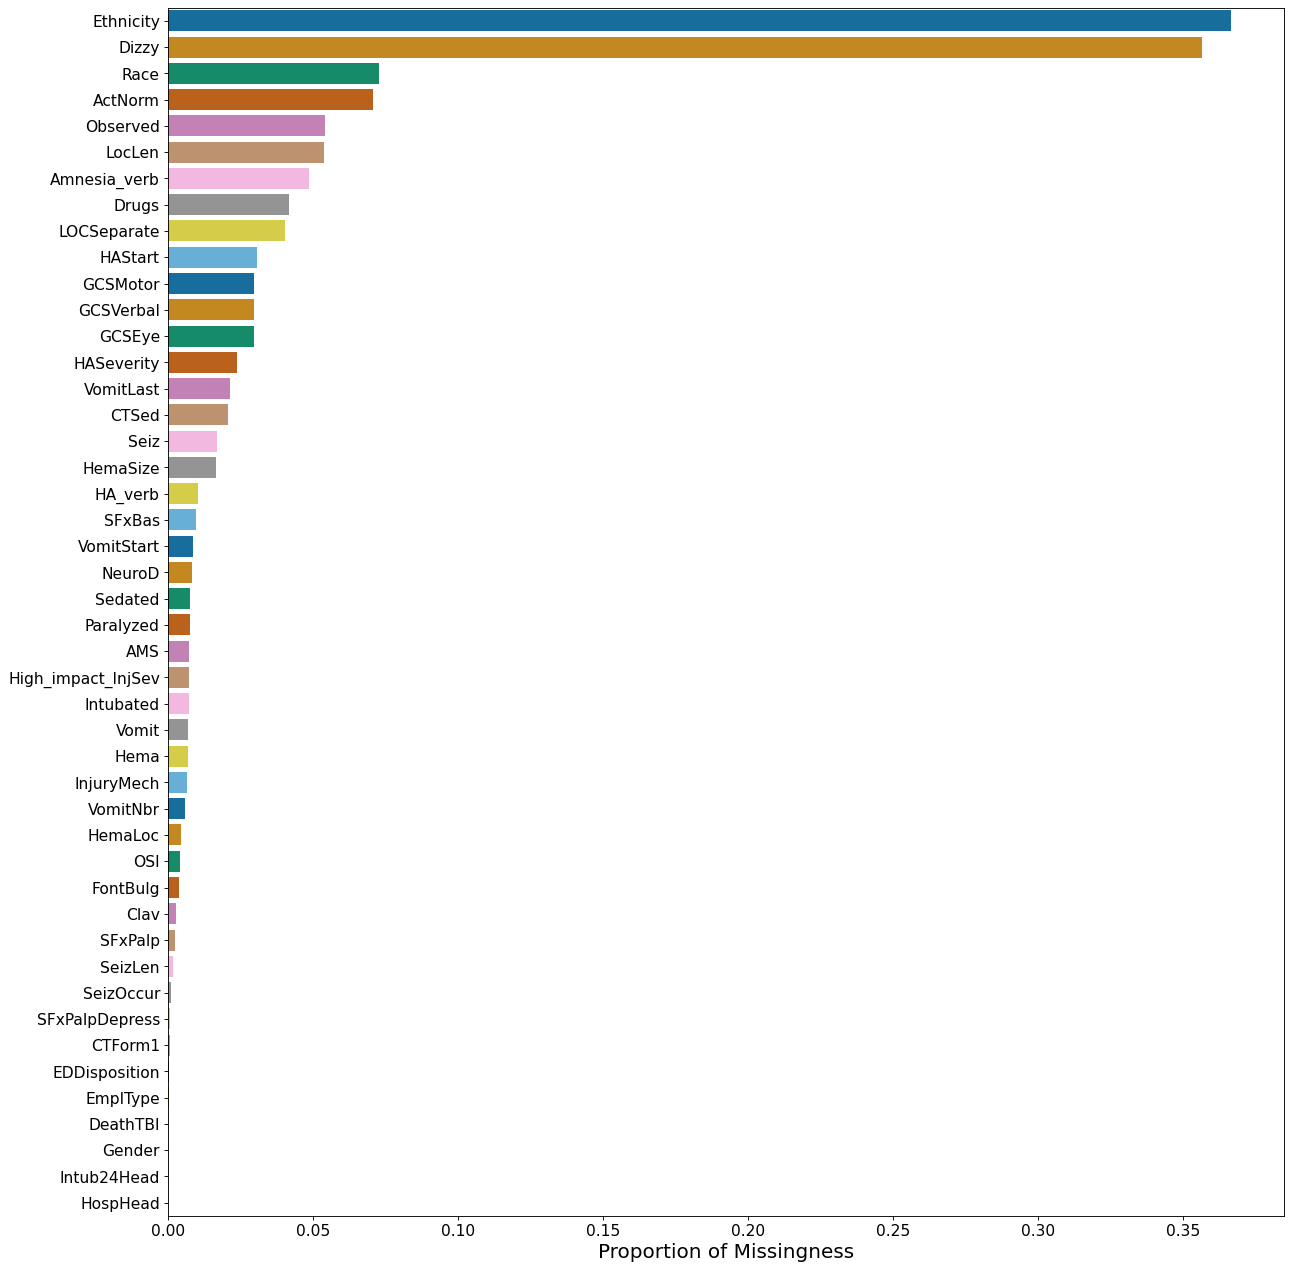
\includegraphics[width=0.5\textwidth]{covariate_missingness.png}
	\caption{Feature Missingness}\label{fig:cov_missing}
\end{figure}

\begin{figure}
	\centering
	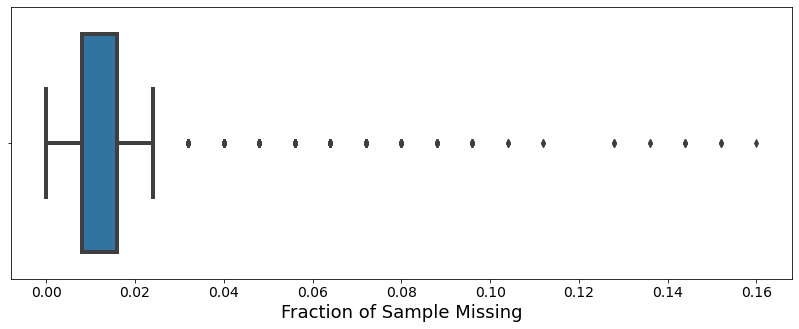
\includegraphics[width=0.5\textwidth]{sample_missingness.png}
	\caption{Sample Missingness}\label{fig:sample_missingness}
\end{figure}
\FloatBarrier

\subsubsection{Age Class Cutoff}

The age was a major factor in [CITE] in terms of creating a decision rule. Two rules were created based on age categories of $< 2$ and $\geq 2$. We can see a large portion of the patient population in our data set is younger and around 2 years of age in Figure \ref{fig:age_dist}.
\FloatBarrier
\begin{figure}
	\centering
	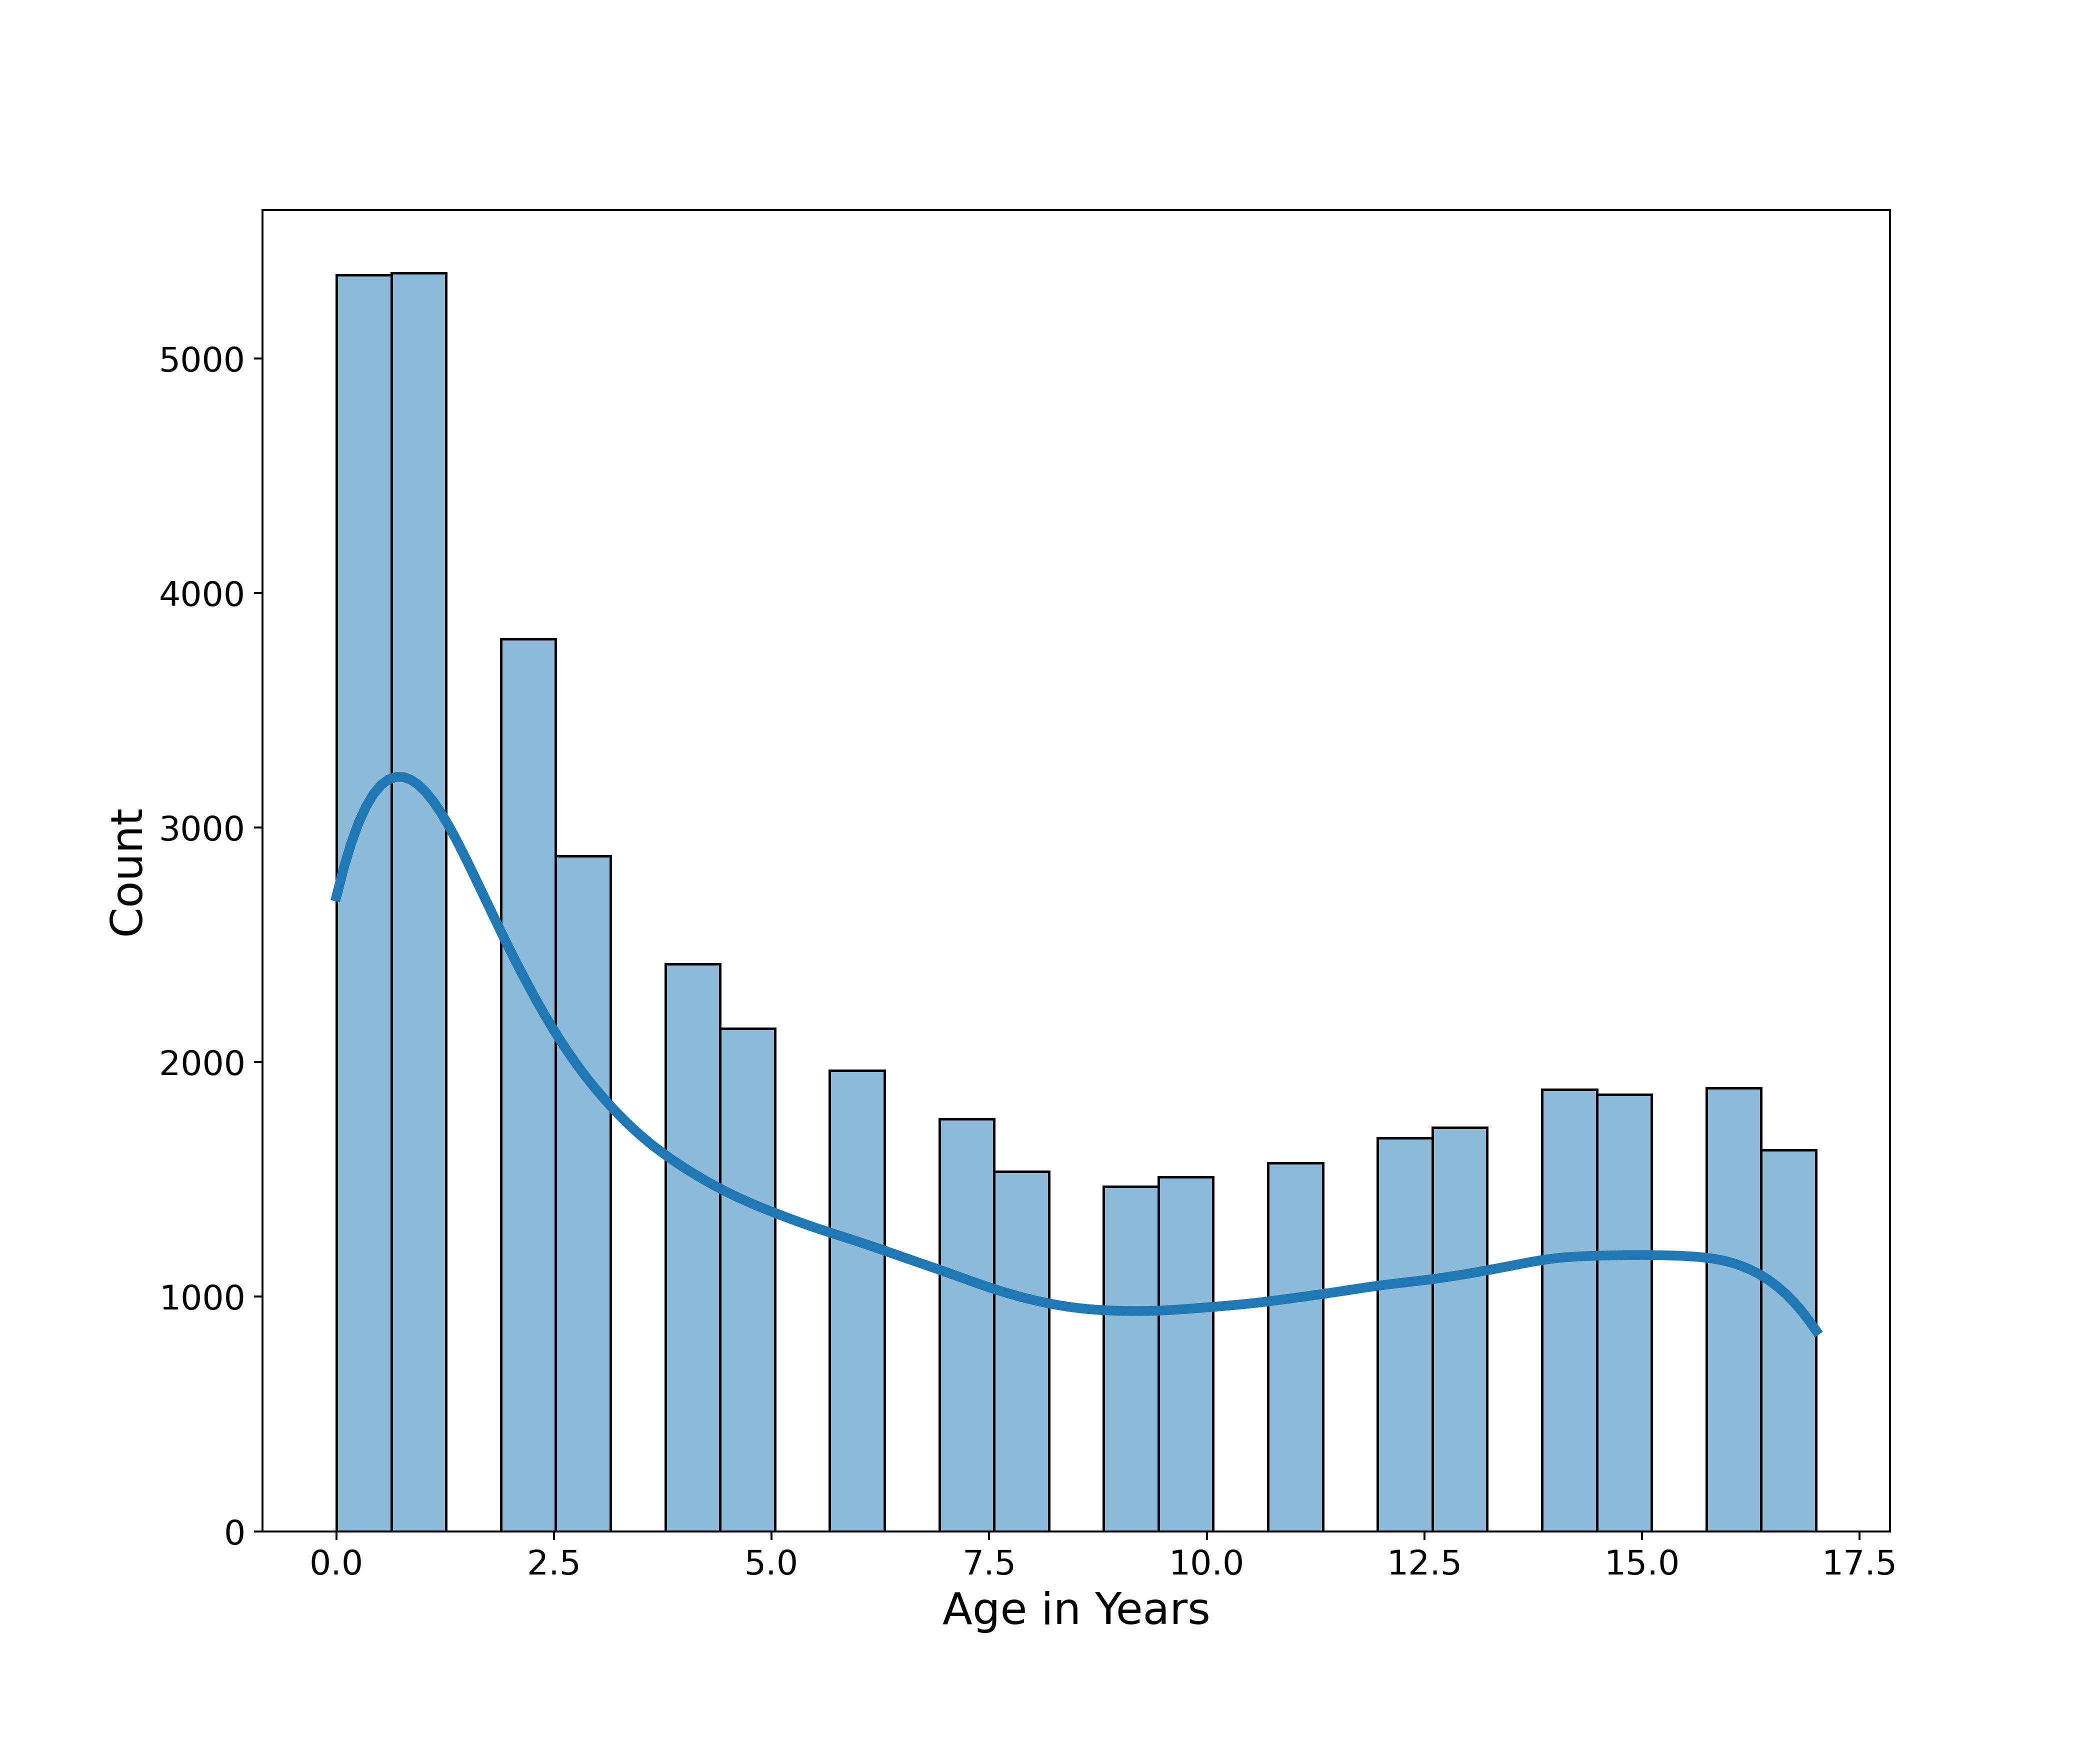
\includegraphics[width=0.5\textwidth]{age_dist.png}
	\caption{Age Distribution with Gaussian KDE}\label{fig:age_dist}
\end{figure}
\FloatBarrier

We want to check the number of pre-nonverbal subjects at each age to see if two years old is a good cutoff age for being verbal, however. Below, in figure \ref{fig:preverbal}, we can see that actually there are still a large proportion of subjects that are pre-verbal at ages 2 and 3 when calculated based on responses for whether a patient had a headache or amnesia in the data. Both of these features are the closest proxy we have to knowing how many pre-verbal patients are in our data set as a binary variable for being pre-verbal does not exist. It is reassuring that the proportions between the two for age age are extremely similar.
\FloatBarrier
\begin{figure}
	\begin{minipage}[b]{0.5\linewidth}
		\centering
		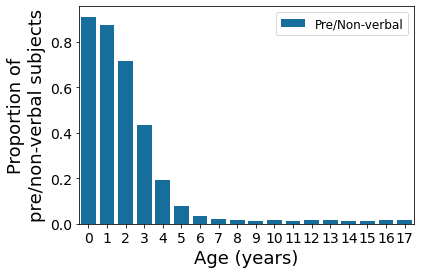
\includegraphics[width=\textwidth]{amnesia_preverbal.png}
		\subcaption{Preverbal response to Amnesia question}\label{fig:amnesia_preverbal}
	\end{minipage}%
	\begin{minipage}[b]{0.5\linewidth}
		\centering
		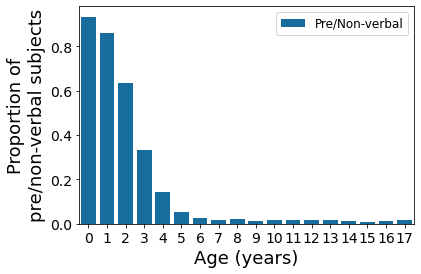
\includegraphics[width=\textwidth]{headache_preverbal.png}
		\subcaption{Age by Injury Severity}\label{fig:headache_preverbal}
	\end{minipage}
	\caption{Preverbal response to Headache question}\label{fig:preverbal}
\end{figure}
\FloatBarrier


\subsubsection{Distribution of Features by Age}

Next, we look at the occurrence of ciTBI in each of our two age categories in Figure \ref{fig:age_by_outcome}. We can see that the proportion of ciTBI in each age category is very close to being the same. The proportions looking at injury severity in Figure \ref{fig:age_by_injury_severity} are similar across age category.
\FloatBarrier
\begin{figure}
	\begin{minipage}[b]{0.5\linewidth}
		\centering
		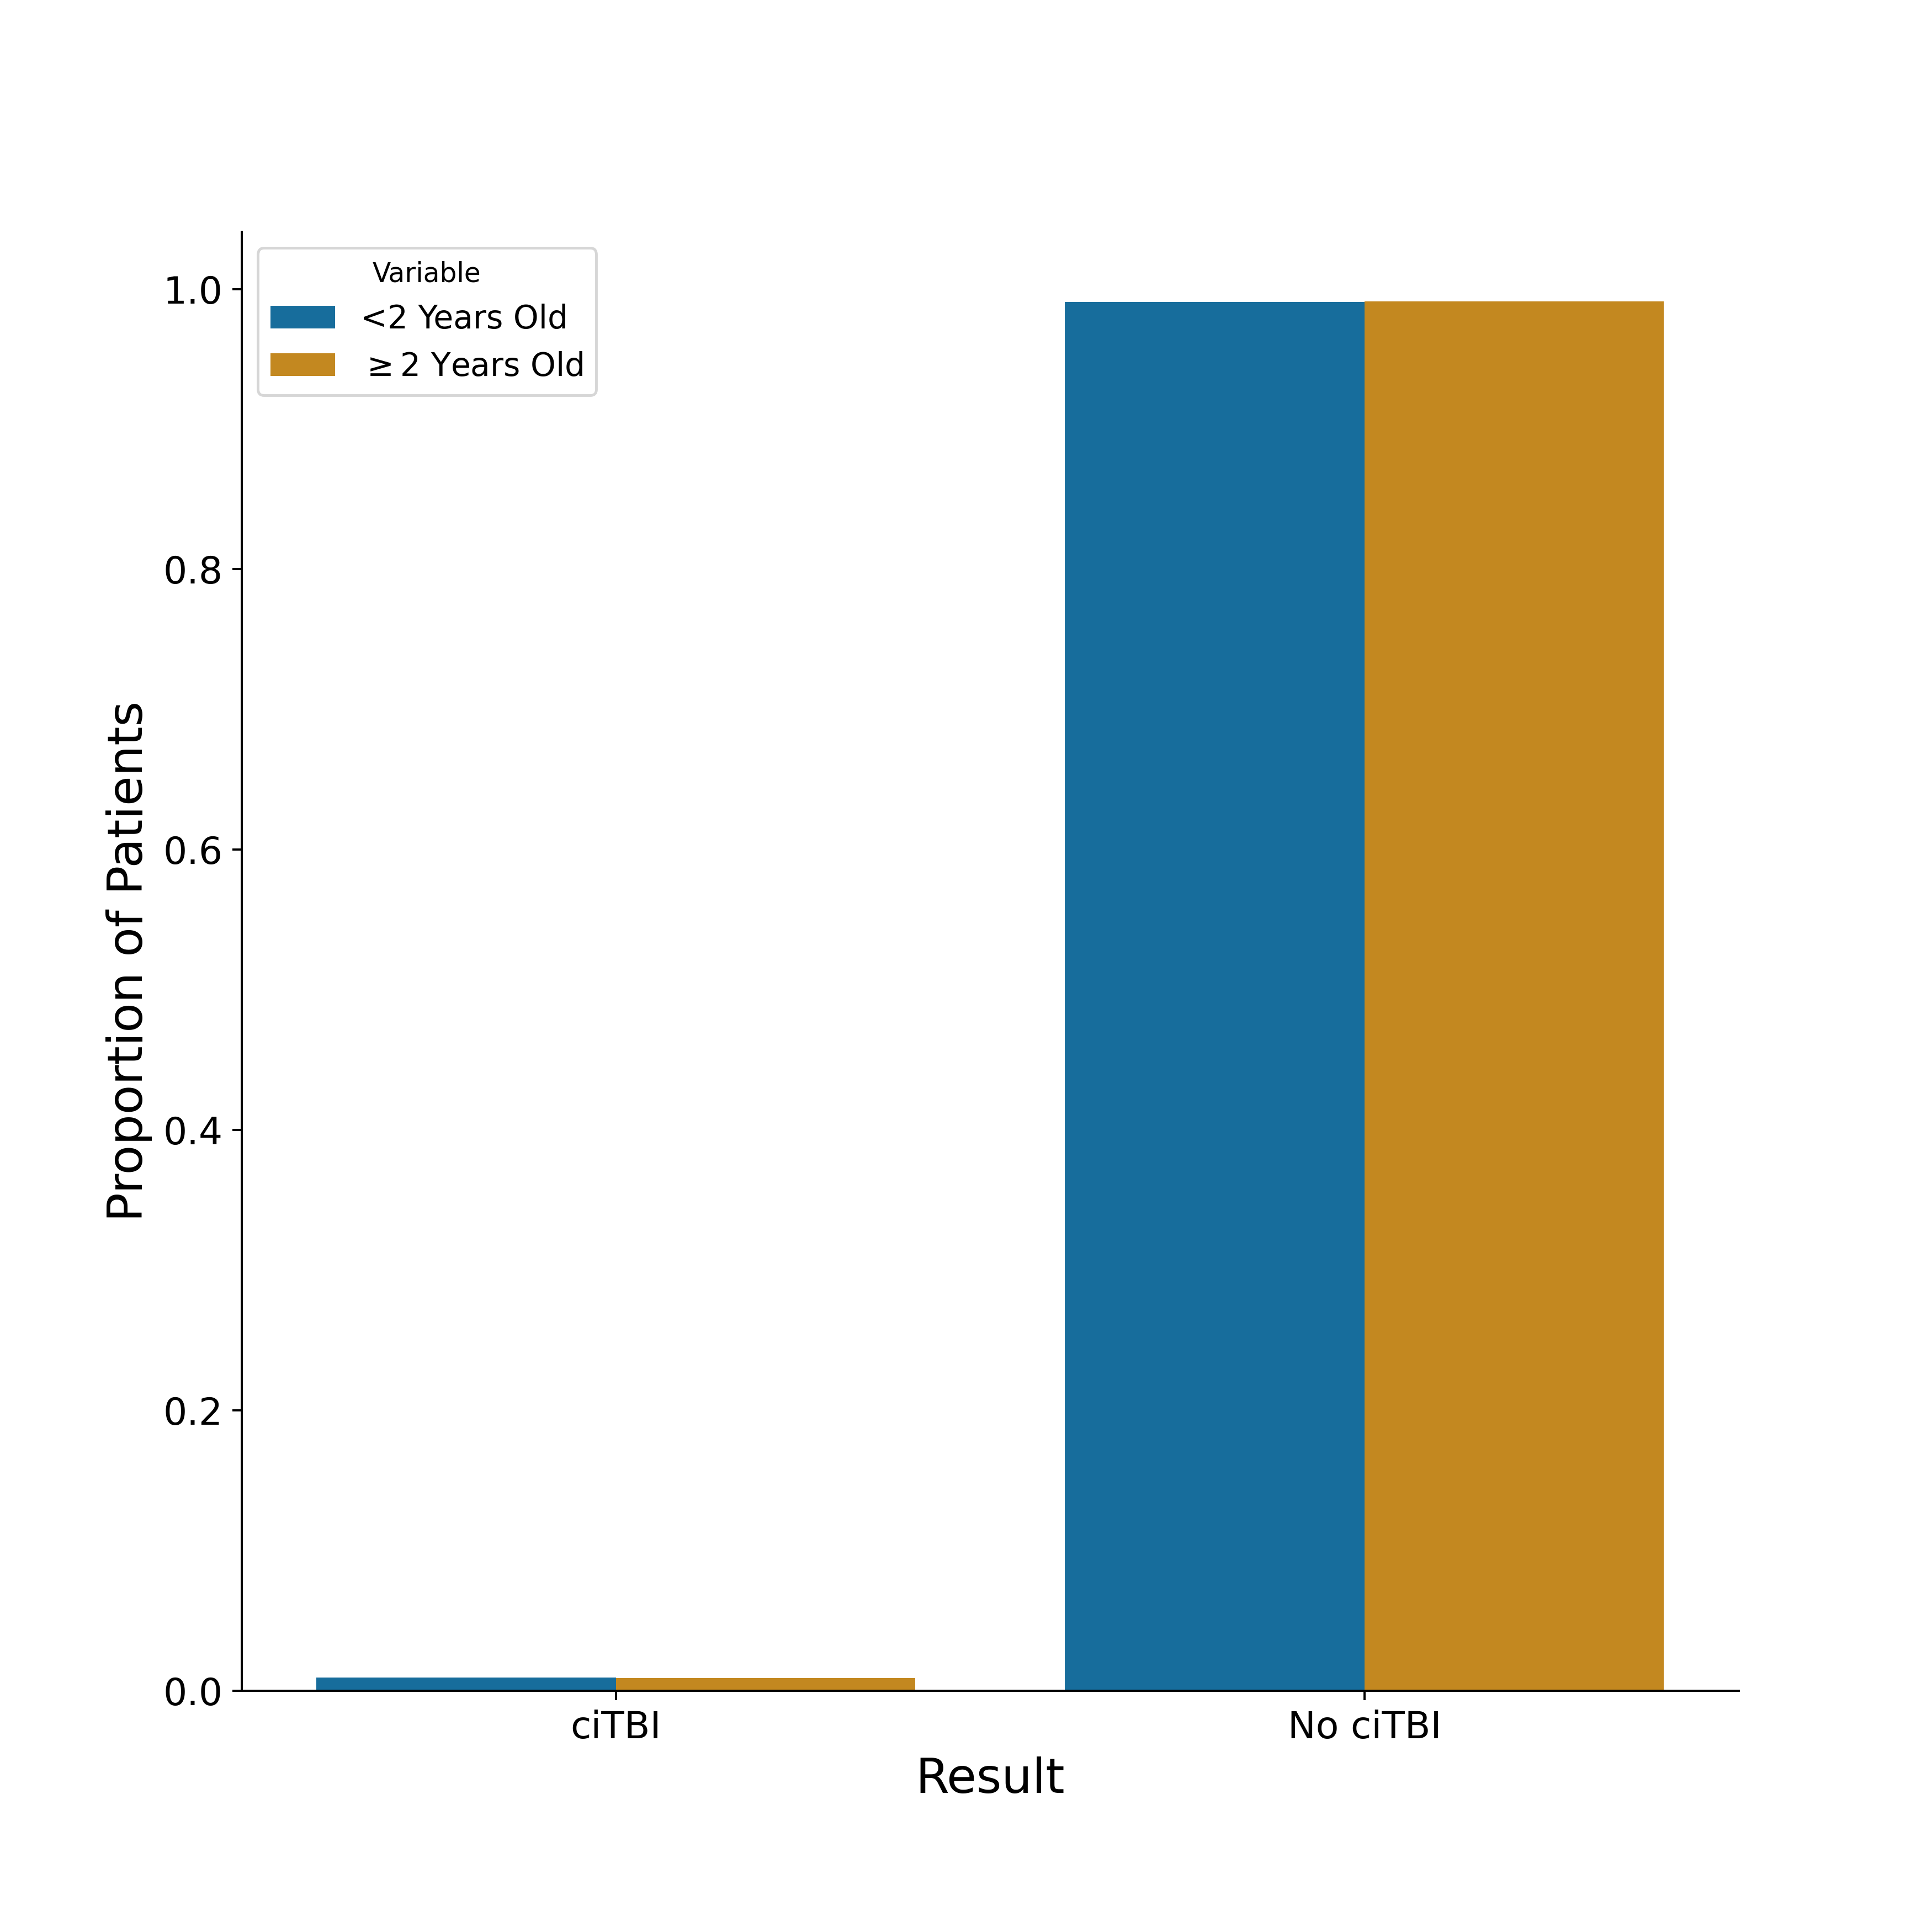
\includegraphics[width=\textwidth]{age_comparison_by_group.png}
		\subcaption{Age by Outcome}\label{fig:age_by_outcome}
	\end{minipage}%
	\begin{minipage}[b]{0.5\linewidth}
		\centering
		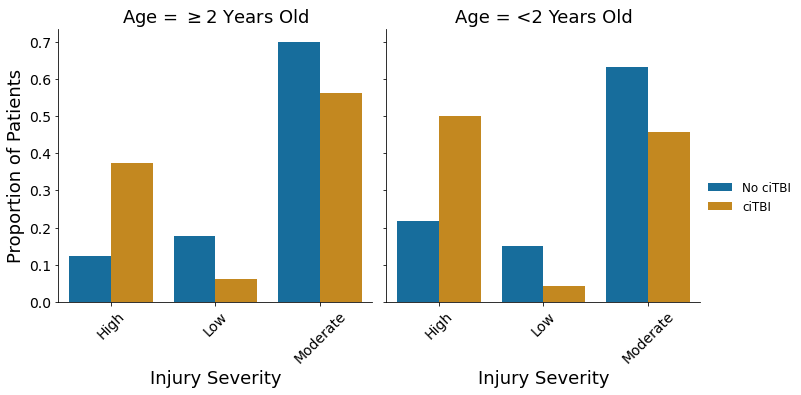
\includegraphics[width=\textwidth]{age_by_injuryseverity.png}
		\subcaption{Age by Injury Severity}\label{fig:age_by_injury_severity}
	\end{minipage}
	\caption{Age broken out by Outcome and Injury Severity}\label{fig:age_distributions}
\end{figure}
\FloatBarrier

However, there may still be other variables with different proportions of positive ciTBI across age categories in Figure \ref{fig:age_covariate}. That is, for each age category and for each outcome, we look at the proportion of patients with the indicated symptom. This exercise might be indicative as to whether such a variable would potentially lead to a different decision rule between the two groups. We can see that the proportion of patients with ciTBI are noticeably different between age $<2$ and age $\geq 2$ for 'Vomit' and 'OSI' (other non-head injury). Also, remember that the variables measuring amnesia and headache cannot be answered by those that are pre-verbal and thus may be useful in a decision rule for those over age 2 but not under.
\FloatBarrier
\begin{figure}
	\centering
	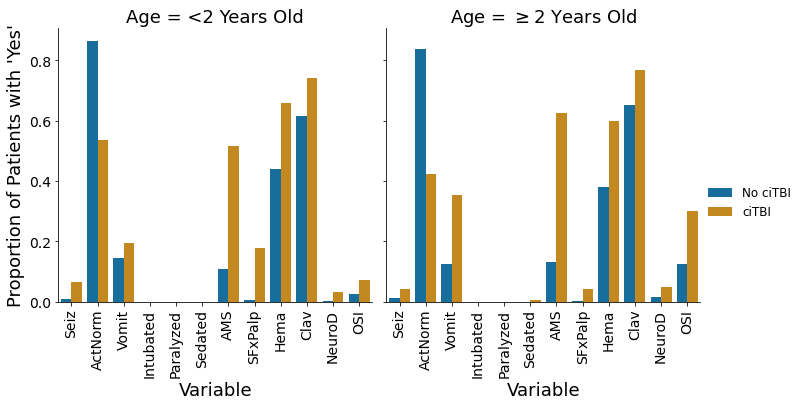
\includegraphics[width=\textwidth]{covariate_by_age.png}
	\caption{Proportion of ciTBI in features split up by age}\label{fig:age_covariate}
\end{figure}
\FloatBarrier

\subsubsection{Correlation of Features to Outcome}

Next, we examine whether any of the features are particularly correlated to the outcome by calculating the Spearman's $\rho$ coefficient on the ordinal variables against the binary outcome. We can see in Figure \ref{fig:spearman_corr_to_outcome} that none of the features are particularly highly correlated with the outcome. A maximum correlation coefficient of 0.12 is attained by the altered mental state feature.
\FloatBarrier
\begin{figure}
	\centering
	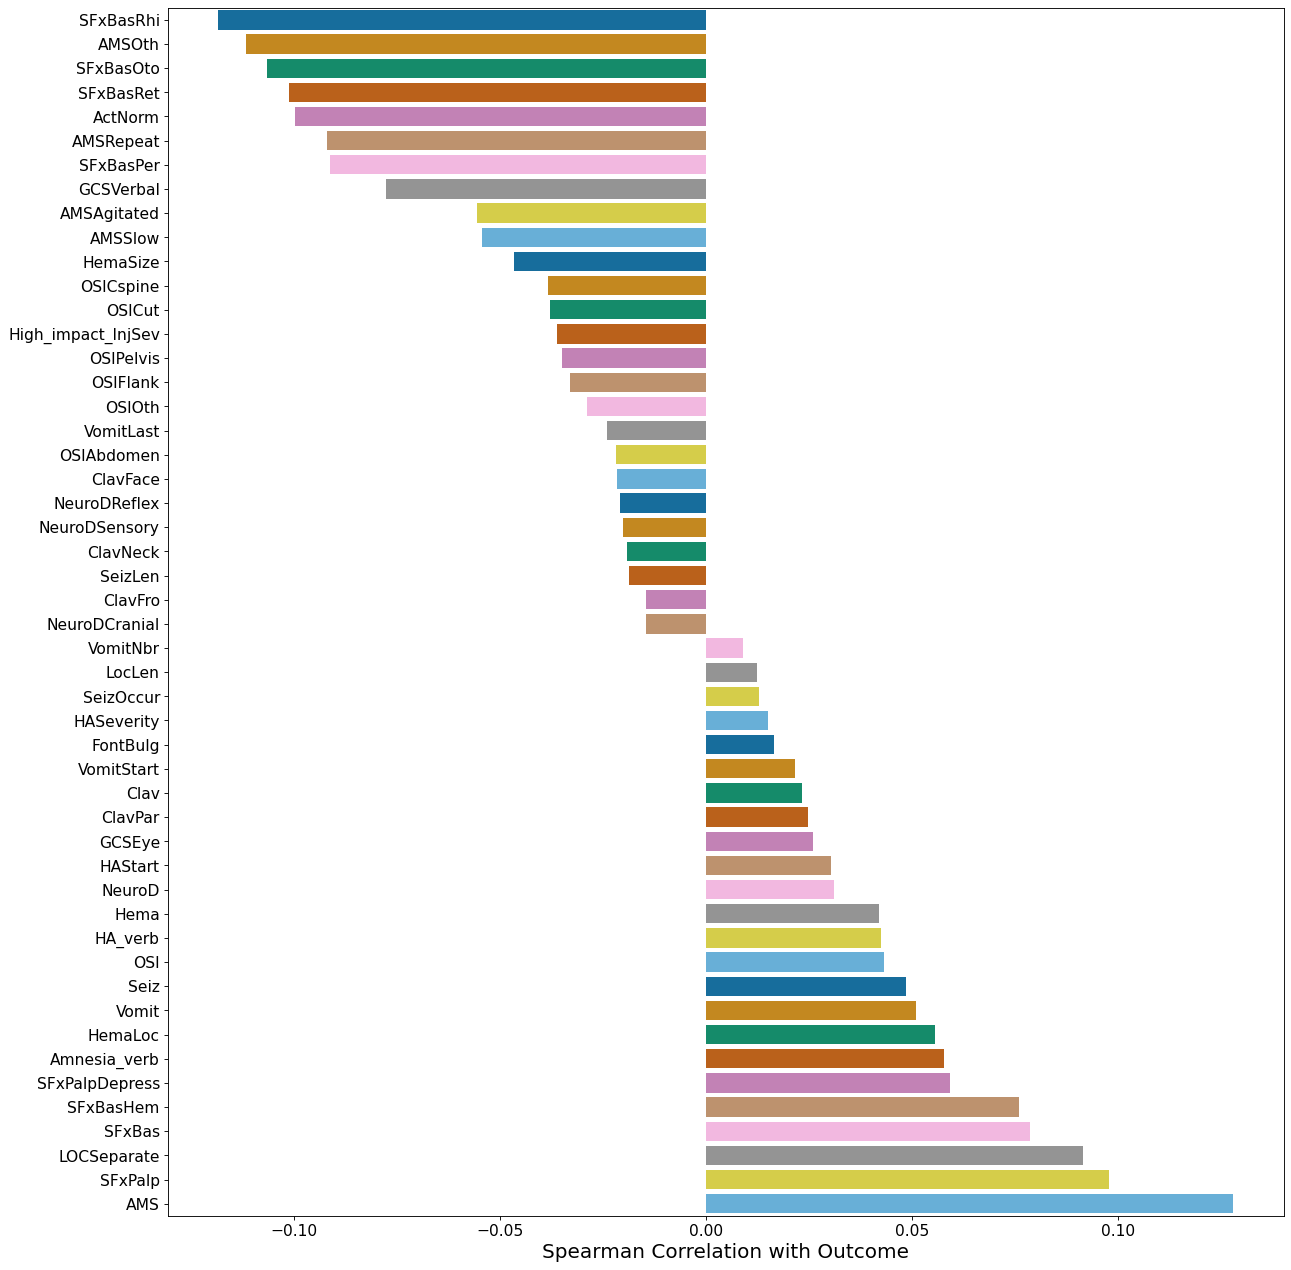
\includegraphics[width=0.5\textwidth]{spearman_corr_to_outcome.png}
	\caption{Spearman Correlation of Features to Outcome}\label{fig:spearman_corr_to_outcome}
\end{figure}
\FloatBarrier

\subsubsection{Principal Component Analysis}

We perform Principal Component Analysis (PCA) on the one-hot encoded data. In Figure \ref{fig:pca_cum_var}, we see that the nearly all of the variance is explained by the first 100 components, and that the first few components capture most of the variance (the first two components explain 13\%, the first five explain 30\%, and the first twenty explain 50\% of variation in the data). That is, noting that the PCA eigenvalues (variances) decay rapidly, we might believe that this dataset behaves like a low-rank signal plus noise. 

In Figure \ref{fig:pca}, we project the one-hot encoded data to two dimensions to study if the classes (age and outcome) are visually separable. First, we see that the classes do not separate, but that there are two distinct clusters in the data---since the data were taken from 25 hospitals, we did not suspect a batch effect. Instead, we see that the presence of an OSI (other, non-head-related injury) leads to the two clusters. Note that the prevalence of OSI in the data is low (10\%), but that it is enough to strongly affect the results of PCA. We will keep this in mind when doing our analyses and look to see if the majority of the misclassified points come from patients who had an OSI injury. This means we may want to consider forming a separate decision rule for this subgroup of the patient population.
\FloatBarrier
\begin{figure}
	\centering
	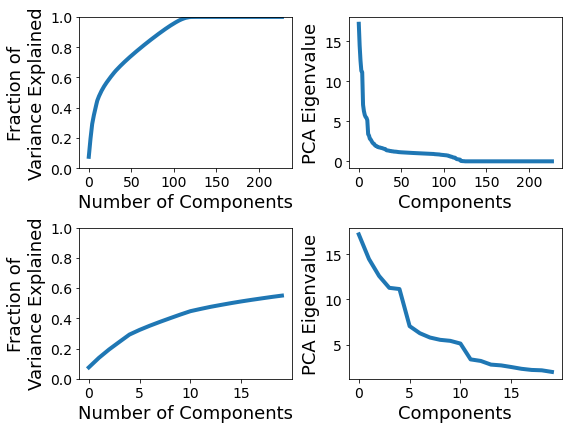
\includegraphics[width=\textwidth]{pca_cum_var.png}
	\caption{Cumulative Variance Explained and Eigenvalues}\label{fig:pca_cum_var}
\end{figure}

\begin{figure}
	\begin{minipage}[b]{0.5\linewidth}
		\centering
		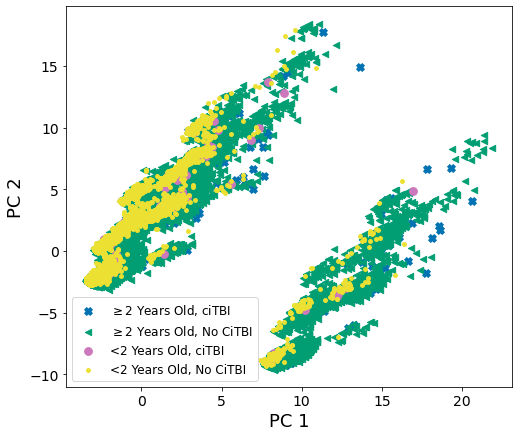
\includegraphics[width=\textwidth]{pca_age_outcome.png}
		\subcaption{PCA colored by Age and Outcome}\label{fig:pca_age_outcome}
	\end{minipage}%
	\begin{minipage}[b]{0.5\linewidth}
		\centering
		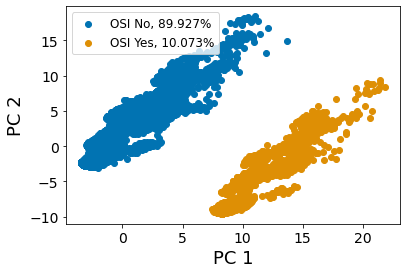
\includegraphics[width=\textwidth]{pca_osi.png}
		\subcaption{PCA colored by OSI}\label{fig:pca_osi}
	\end{minipage}
	\caption{Age Figure}\label{fig:pca}
\end{figure}
\FloatBarrier

\section{Baseline Model}

%In this section, we will discuss how exactly we decided to reformulate the baseline model as described in the paper. As discussed in the EDA section, we ensured that we were starting with the same data - as noted we found 20 missing outcomes instead of 18, but aside from this we found the data to match up nicely. To further replicate the data used, we noticed the paper transformed several variables to be binary - 'HemaLoc', 'LocLen', 'High\_impact\_InjSev', 'HASeverity', 'SeizLen', 'HemaSeize', 'LOCSeparate', and 'SFxPalp'. The paper binned several categories of these features together into 'Yes' and 'No' which they describe in the decision tree visuals created. After making this change, we partition the data into two groups - those with kids less than two years old and one for those that are greater than or equal to two. From here, to mimic the same results we use the same features derived in the paper alongside the same depth and class imbalances. Oddly enough, they cite weights of 500:1 "for failure to identify a patient with ciTBI versus incorrect classification of a patient without ciTBI". The intuition for this weighting scheme is due to the imbalances in the classes to begin with however the exact cost is rather arbitrary. Anyhow, with this in mind, we fit the two decision rules - one for young and one for old kids. The plot for children less than two is interesting as it does not match what the paper found whatsoever in terms of the order of important features while the second tree shows comparable important features. As far as scores are concerned, we obtain the following metrics (young model, old model) - AUC: (0.855, 0.853), Accuracy: (0.854, 0.853), Sensitivity: (0.855, 0.833), Specificity: (0.789, 0.796), and Balanced Accuracy: (0.822, 0.814). 

\section{Modeling}

We ran decision trees, boosting methods such as AdaBoost and LogitBoost, logistic regression, and an SVM on our data set in order to determine which had the best performance. 

\section{Conclusions}
asdf.

\subsection{Division of Labor}
asdf.

\section{References}

\end{document}  
